% ======================================================================================================
% NOTES, TODOS
% ======================================================================================================
\subsection{Search Result and Bibliometric Analysis}
Following the selection process using the inclusion and exclusion criteria, and the removal of duplicate studies, a total of 74 research papers were considered for further review and analysis. Of these, 44(60\%) were conference papers, while the remaining 40\% were journal articles.

The Majority of the selected papers were retrieved from Web of Science and Scopus, with approximately 41\% and 23\% respectively, as both are the major citation databases. Furthermore, a notable proportion of papers were also obtained from other sources, including the IEEE Digital Library (15.1\%), Springer Link (11\%), ACM Digital Library (6.8\%), and Science Direct (2.7\%). These finding are illustrated in Figure \ref{fig:archive-itemtype}, using pie chart in terms  of document type and source archive. These chart highlight the importance of leveraging a wide range of digital archives to ensure a comprehensive review of the literature. 

% \begin{figure}
% \includesvg[width=0.5\textwidth]{images/svg/databases.svg}
% \includesvg[width=0.5\textwidth]{images/svg/itemtype.svg}
% \svgcaption{This is the label for the SVG image.}
% \label{fig:image}
% \end{figure}

\begin{figure}[H]
    \centering
    \begin{subfigure}[b]{0.45\textwidth}
        % \includegraphics[width=\textwidth]{image1.png}
        \includesvg[width=\textwidth]{images/svg/databases.svg}
        \caption{Percentage of papers per database}
    \end{subfigure}
        \begin{subfigure}[b]{0.45\textwidth}
        % \includegraphics[width=\textwidth]{image2.png}
        \includesvg[width=\textwidth]{images/svg/itemtype.svg}
        \caption{Proportion of papers per item type}
    \end{subfigure}
    \caption{Paper distribution}
    \label{fig:archive-itemtype}
\end{figure}


Analysis of the distribution of selected papers based on publication year revealed that the majority of articles were published in 2022 and 2021. Furthermore, the bar chart illustrates a general upward trend in the number of publications addressing security concerns for industries utilizing Digital Twin and (I)IoT applications. This trend indicates that there is a growing interest and concern among researchers in the field of Digital Twin and IoT security, and highlights the relevance and timeliness of this systematic literature review.

\begin{figure}[H]
    \includesvg[width=0.9\textwidth]{images/svg/pub_year_white_bg.svg}
    \caption{Number of published papers per year}
    \label{fig:bar-chart-yaer}
\end{figure}
% \hajj{please remove the background color of the figure}
To gain a deeper understanding of the trending topics within the 74 selected papers published between 2018 and 2023, a frequency analysis of keywords was conducted. This analysis was performed by extracting keywords that appeared more than three times in the abstracts and keyword sections of the articles, using the VOSviewer tool. Further filtering and sensitization was applied to create a shortlist of keywords. Additionally, keywords which have similar meanings with different spellings and variations were merged. The resulting frequency analysis of keywords, illustrated in Figure \ref{fig:alluvial-key}, provides valuable insights into the key themes and concepts that are prevalent in current research on the topic of Digital Twin and IoT security. This analysis can help guide future research by identifying areas where there is a need for further investigation and providing a sense of the current state of the field.


\begin{figure}[H]
    % \includesvg[width=0.9\textwidth]{images/svg/key_buble.svg}
    % 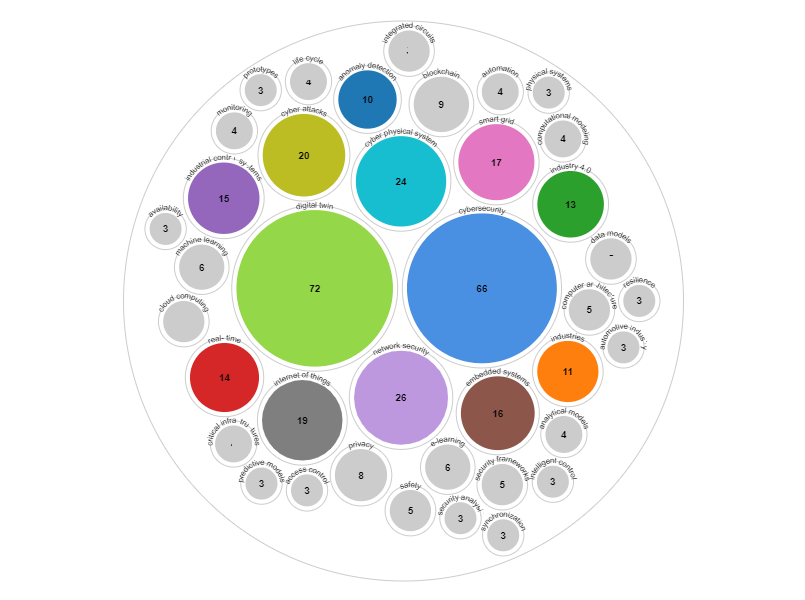
\includegraphics[width=\textwidth]{images/svg/key_buble.png}
    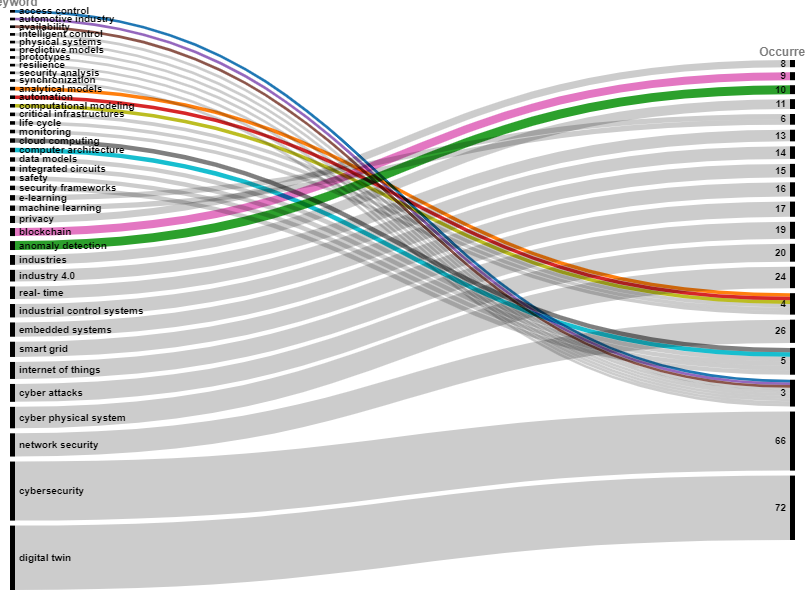
\includegraphics[width=\textwidth]{images/key_belt.png}
    \caption{Frequency of keywords}
    \label{fig:alluvial-key}
\end{figure}

Bibliographic information from 175 papers is used to generate 1187 keywords. Using thesaurus text file, we configure the tool to merge keywords that have similar semantic meaning. Moreover, we set a minimum threshold to limit the result to 87 keywords that meet 3 occurrences of the 1187 keywords.    


The analyisis of the selected papers using VOSviewer software revealed that which terms were frequently mentioned on the abstract and keyword section of the paper. The most frequently mentioned terms were "digital twin" with 72 occurrences, followed by "cybersecurity" with 66 occurrences, "cyberphysical system" with 24 occurrences, "cyber attacks" with 20 occurrences, "internet of things" with 19 occurrences, and "embedded systems" with 17 occurrences.This analysis highlights the key themes and concepts that are prevalent in current research on the topic of Digital Twin and IoT security. The high frequency of the term "digital twin" indicates the centrality of this concept in the field and the importance of understanding its role in ensuring the security of industries utilizing DT and IoT applications. The frequent mention of terms such as "cybersecurity" and "cyber attacks" further emphasizes the need for robust security measures to protect these systems from malicious actors.Additionally, the presence of terms such as "cyberphysical system" and "embedded systems" highlights the need for interdisciplinary research and collaboration between experts in fields such as computer science, engineering, and physics to effectively address the security challenges facing Digital Twin and IoT.

In order to gain further insights into the evolution of research in the field of Digital Twin and IoT security, a keyword co-relationship network analysis was extracted from VOSviewer tool. This analysis aimed to identify clusters of related items and to visualize the relationships between keywords over time. The results of this analysis revealed that in the early days of research on Digital Twin, keywords such as "monitoring", "safety", "prototypes", "resilience", "software", and "tools" were frequently mentioned, which suggests that the primary focus of research at that time was on utilizing Digital Twin as a visual aid. However, more recent research is characterized by the frequent mention of emerging technologies such as "blockchain," "machine learning," "e-learning" "5G," and "privacy" This indicates that the development of Digital Twin has shifted towards utilizing these technologies to enhance its security capabilities. This highlights the importance of continuous monitoring of the research field and to adapt to new technologies and approaches for Digital Twin security.



\begin{figure}[H]
    % \centering
    % 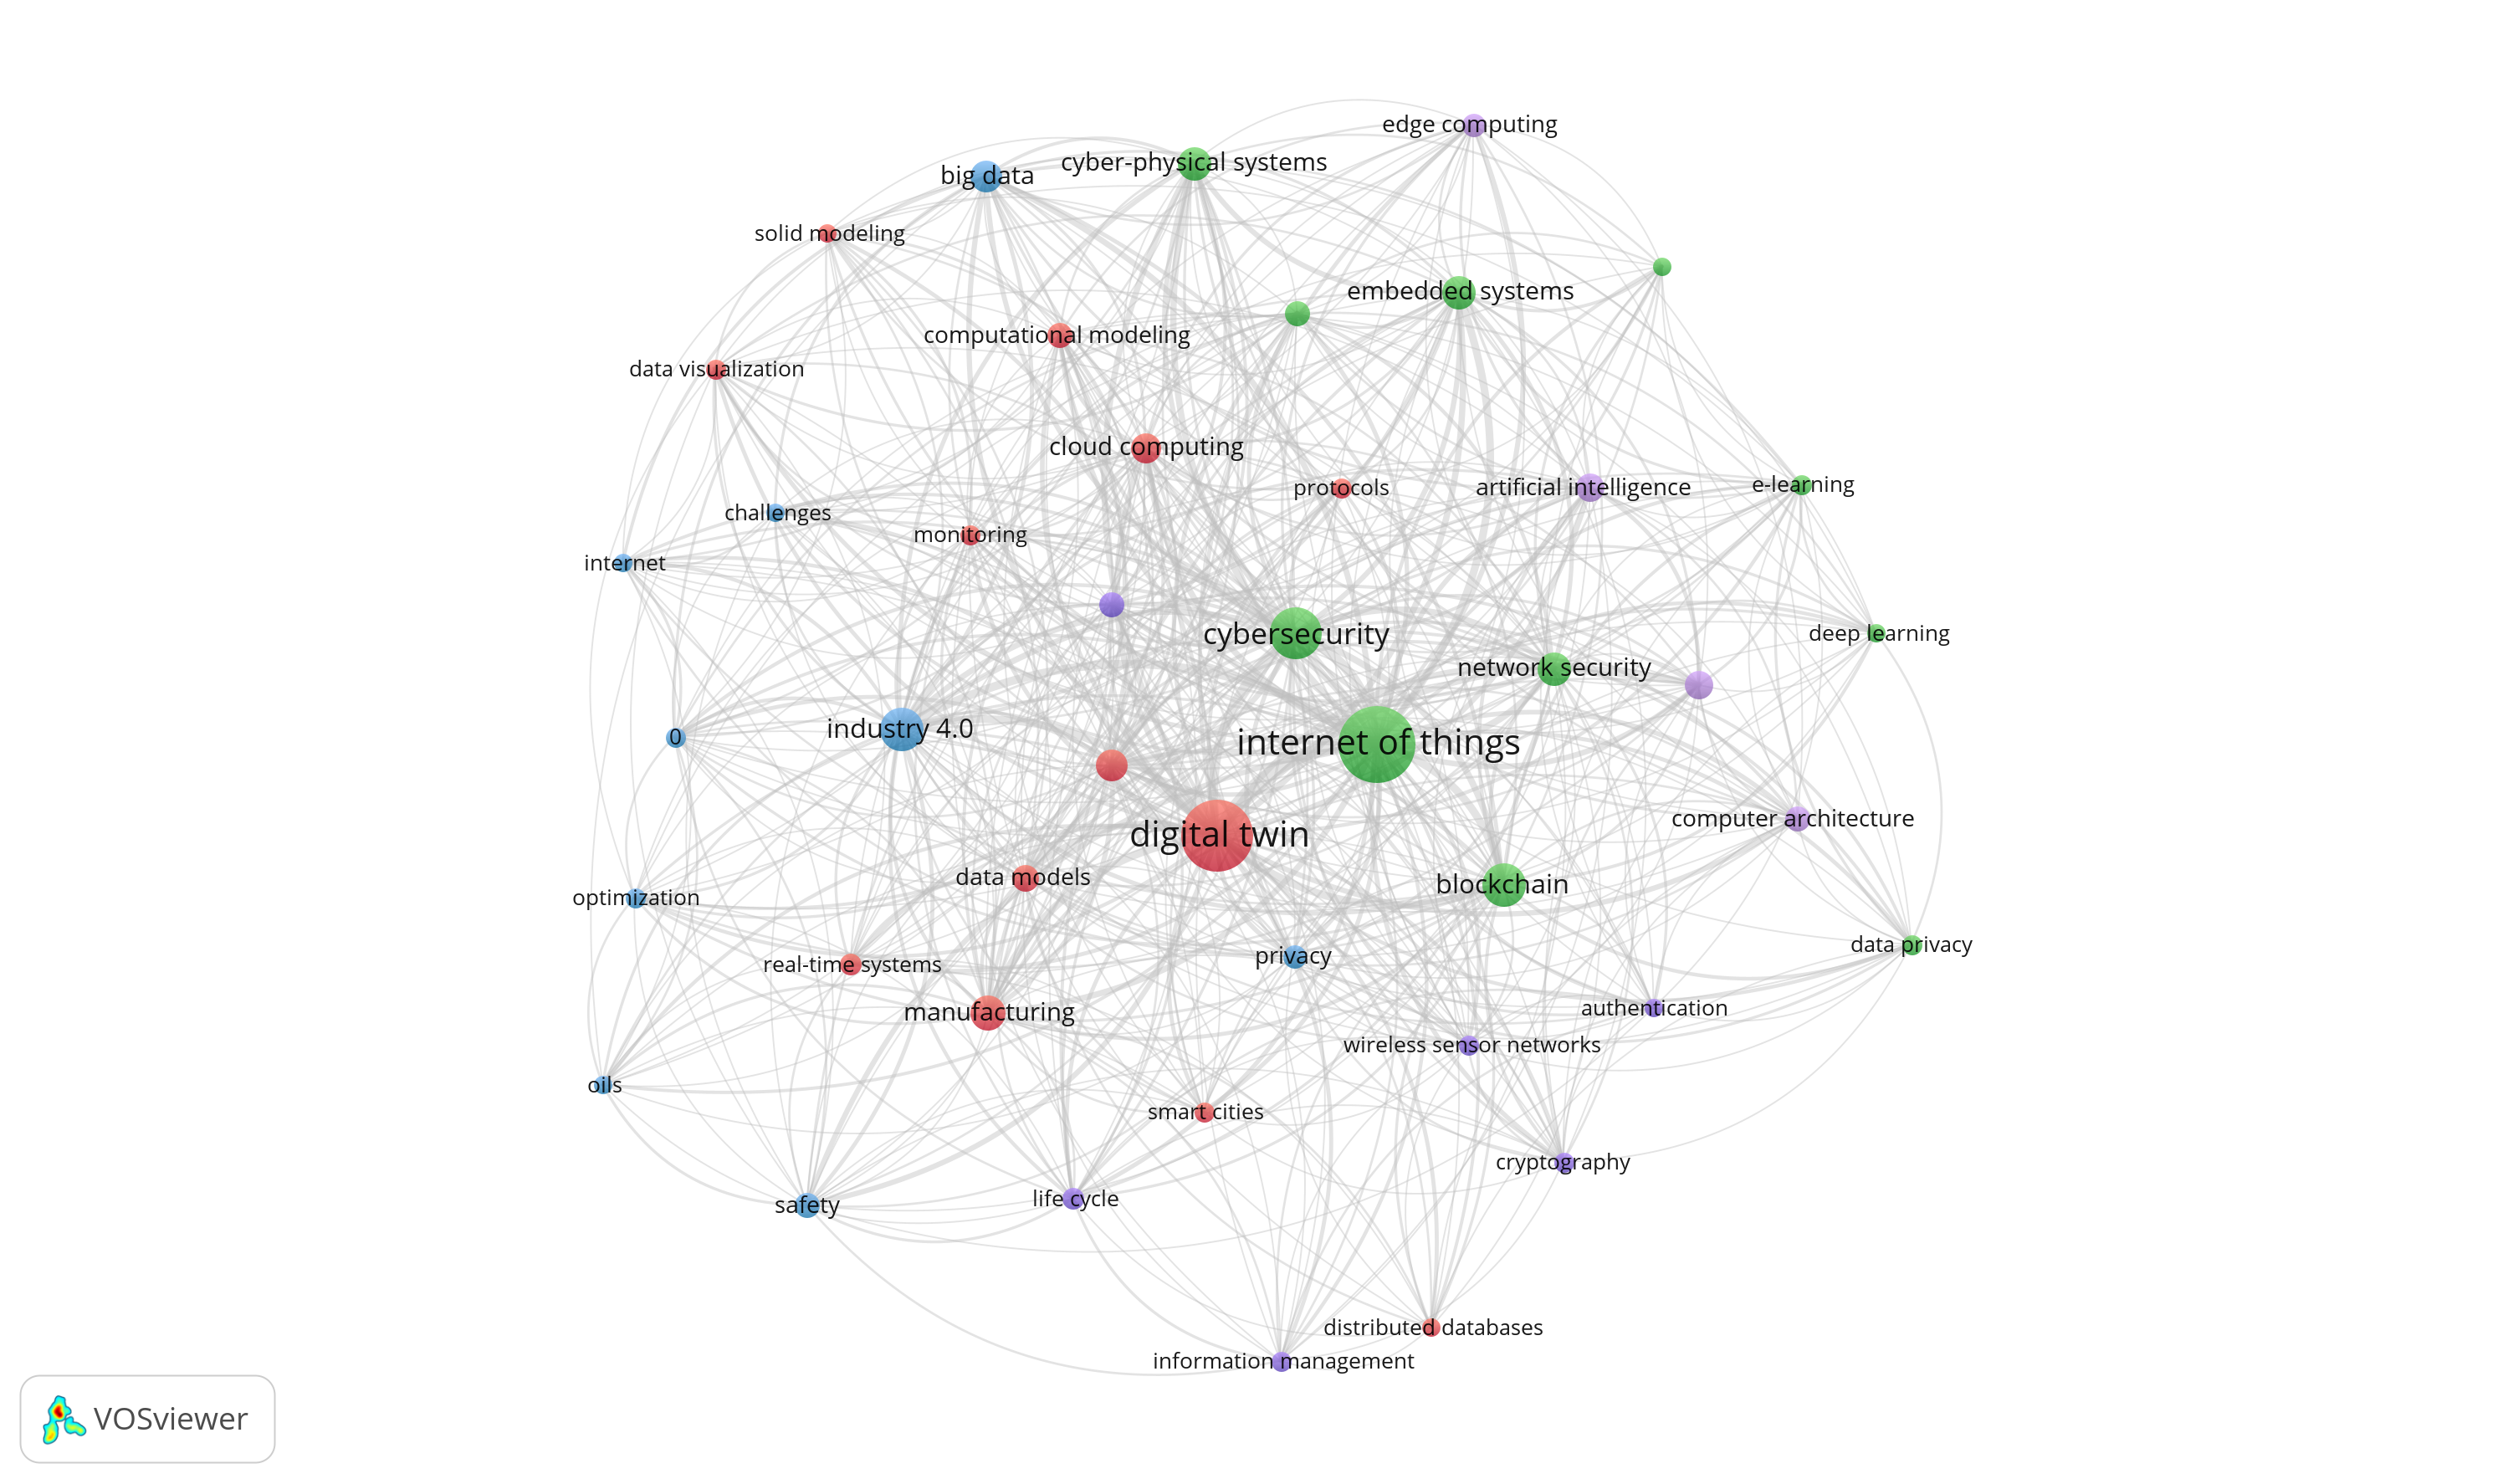
\includegraphics[width=1.5\textwidth, center]{images/vos_key_cooc_6_final.png}
    \includesvg[width=\textwidth]{images/svg/vos_co_time_2.svg}
    % \includesvg[inkscapelatex=false,width=0.95\columnwidth]{images/key_belt.svg}
    \caption{keyword co-relationship from VOSviewer}
    \label{fig:co-occurrence-vosv}
\end{figure}

The analysis of the co-occurrence of keywords in the selected articles, as represented in Figure \ref{fig:co-occurrence-vosv}, reveals the identification of five clusters. These clusters, as defined by the VOSviewer documentation, are groups of terms that exhibit a high degree of relatedness. Cluster one encompasses terms related to 5G technology, machine learning, real-time security analysis, security frameworks, access control, and automation. Cluster two comprises of keywords such as cybersecurity, data models, digital twin, internet of things, privacy, prototypes, safety, and cloud computing. The third cluster encompasses terms such as those related to the automotive industry, availability, blockchain, industry 4.0, industrial control systems, system life cycle, intelligent control, software, and tools. The fourth cluster is comprised of analytical models, anomaly detection, cyber-attacks, monitoring, resilience, critical infrastructure, integrated circuits, and physical systems. The final cluster includes terms such as cyber-physical systems, e-learning, embedded systems, predictive models, and smart grids.